\section{Supplemental figures and tables to main text}

\begin{figure}[ht]

    \includegraphics[width=\textwidth]{../covid_19/projects/sri_lanka/supplementary figures/posterior_distributions.png}
    \textbf{\caption{Histograms of prior (blue lines) and posterior (red bars) distributions for epidemiological parameters for Sri Lanka. In the VoC emergence start time the lower bounds and upper bounds for Alpha and Delta strains correspond to, 29th Jan 2021 to 28th Feb 2021 and 04th May 2021 to 03rd July 2021, respectively.}}
    \label{fig:posterior_distributions}
\end{figure}

\begin{figure}[ht]

    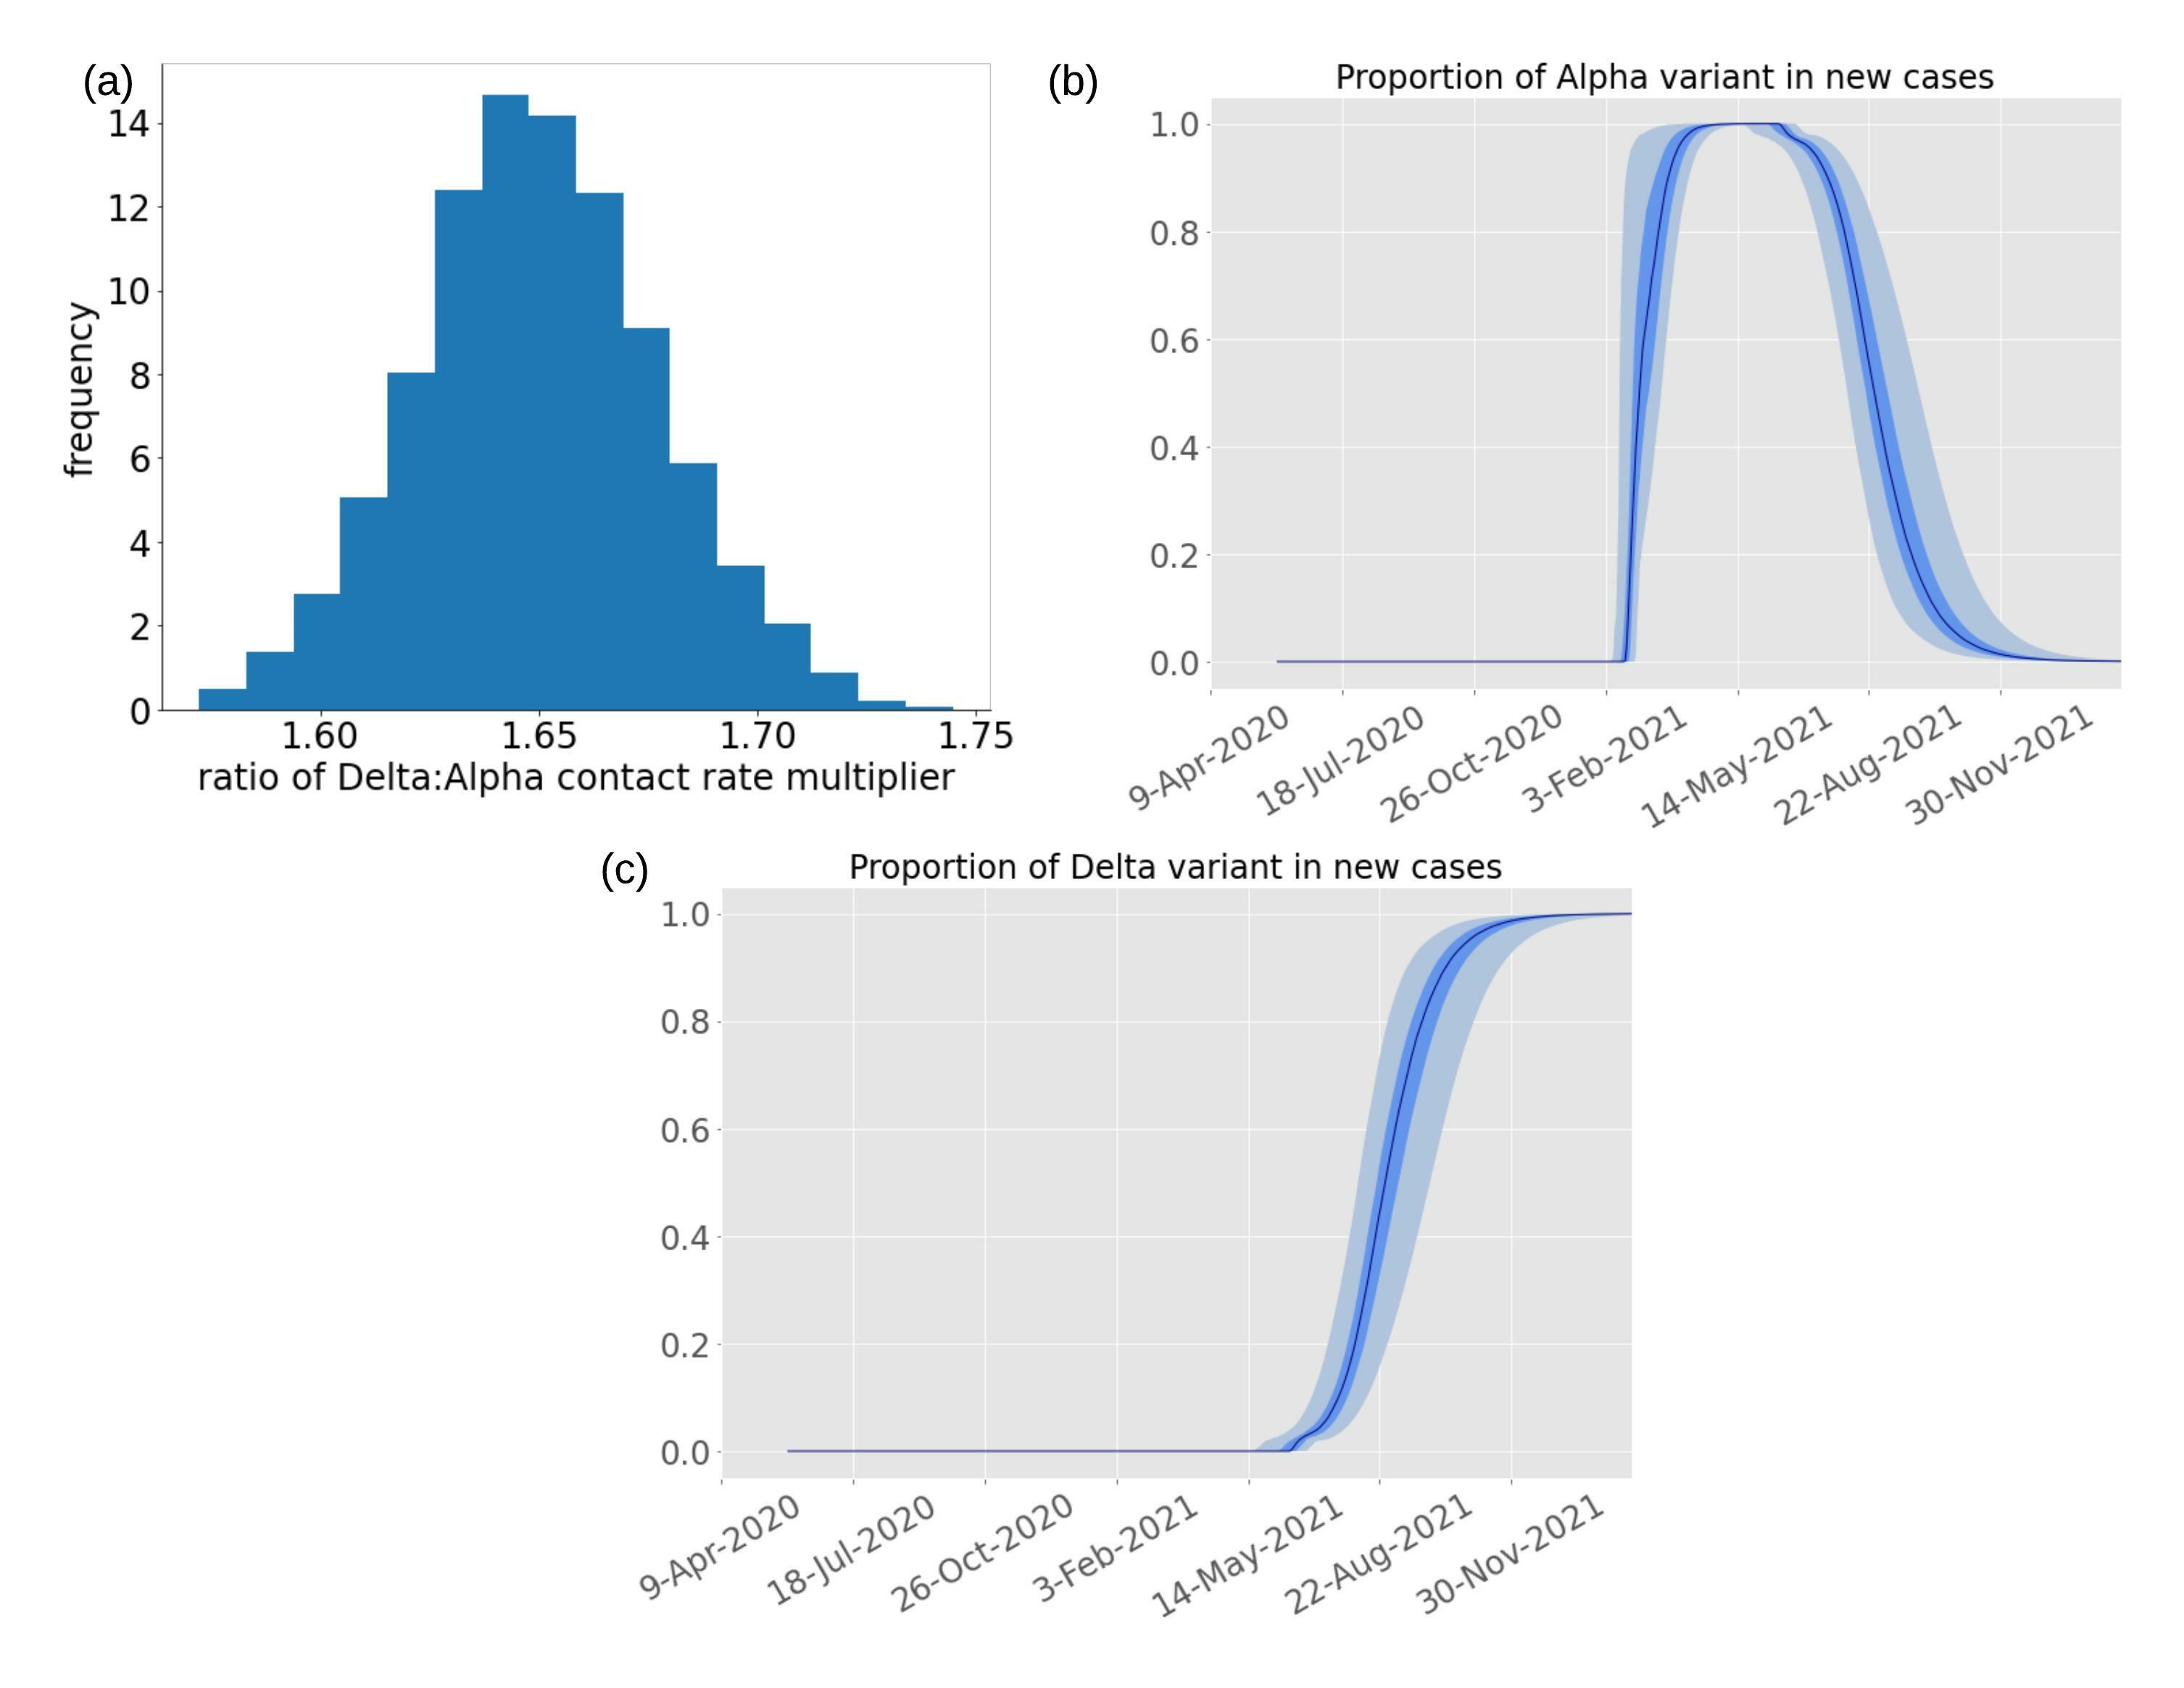
\includegraphics[width=\textwidth]{../covid_19/projects/sri_lanka/supplementary figures/Alpha_Delta.jpeg}
    \textbf{\caption{The ratio of the increased transmissibility of Delta strain to the increased transmissibility of Alpha strain (a), the proportion of Alpha (b) and Delta (c) variants in new cases.}}
    \label{fig:alpha_delta}
\end{figure}

\begin{figure}[ht]

    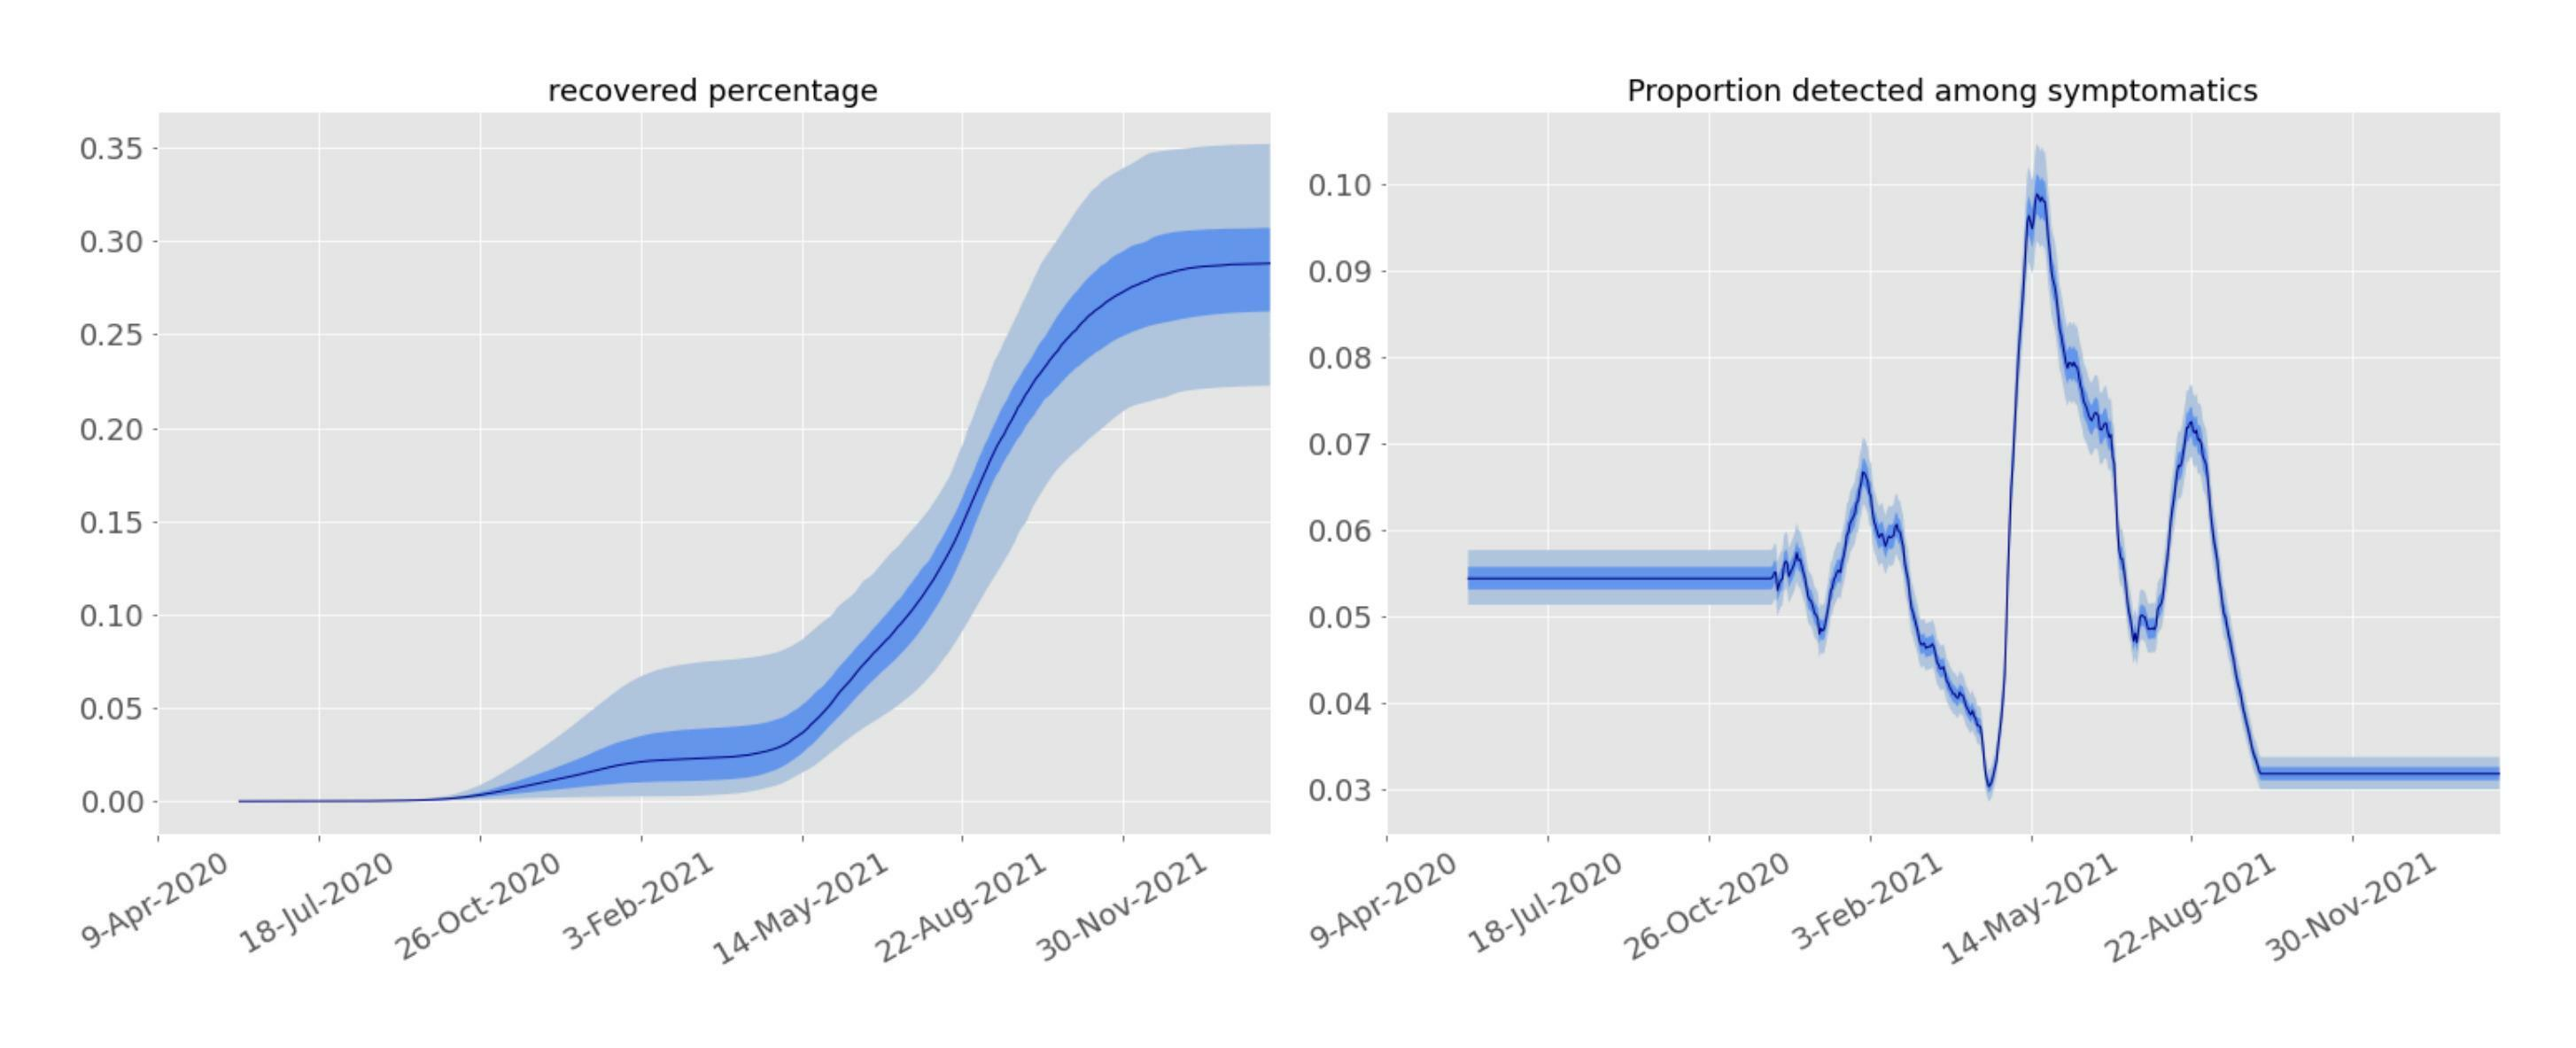
\includegraphics[width=\textwidth]{../covid_19/projects/sri_lanka/supplementary figures/covid_19 - CDR.jpeg}
    \textbf{\caption{The modelled recovered percentage (a) and the model estimated proportion of symptomatic cases (b).}}
    \label{fig:cdr}
\end{figure}